\documentclass[12pt,a4paper]{article}

\usepackage{amsmath,amscd,amsbsy,amssymb,latexsym,url,bm,amsthm}
\usepackage{epsfig,graphicx,subfigure}
\usepackage{enumitem,balance}
\usepackage{wrapfig}
\usepackage{mathrsfs, euscript}
\usepackage[usenames]{xcolor}
\usepackage{hyperref}
\usepackage{multicol}

\theoremstyle{definition}

\newtheorem{theorem}{Theorem}
\newtheorem{lemma}[theorem]{Lemma}
\newtheorem{proposition}[theorem]{Proposition}
\newtheorem{corollary}[theorem]{Corollary}
\newtheorem{exercise}{Exercise}[section]
\newtheorem*{solution}{Solution}

\numberwithin{equation}{section}
\numberwithin{figure}{section}

\renewcommand{\thefootnote}{\fnsymbol{footnote}}

\newcommand{\postscript}[2]
 {\setlength{\epsfxsize}{#2\hsize}
  \centerline{\epsfbox{#1}}}

%changing 1.5 will give you different space between lines.
\renewcommand{\baselinestretch}{1.0}

\setlength{\oddsidemargin}{-0.365in}
\setlength{\evensidemargin}{-0.365in}
\setlength{\topmargin}{-0.3in}
\setlength{\headheight}{0in}
\setlength{\headsep}{0in}
\setlength{\textheight}{10.1in}
\setlength{\textwidth}{7in}


\begin{document}

\noindent\framebox[\linewidth]{\shortstack[c]{
\Large{\textbf{Lab05-Numbering Programs}}\vspace{1mm}\\
CS363-Computability Theory, Xiaofeng Gao, Spring 2016}}
\begin{center}
\footnotesize{\color{red}$*$ Please upload your assignment to FTP or submit a paper version on the next class}

\footnotesize{\color{red}$*$ If there is any problem, please contact: nongeek.zv@gmail.com }

\footnotesize{\color{blue}$*$ Name:Yupeng Zhang \quad StudentId: 5130309468 \quad Email: 845113336@qq.com}
\end{center}


\begin{enumerate}%[topsep=0pt, partopsep=0pt, itemsep=2pt,parsep=2pt]
  \item Show that there is a total computable function $k$ such that for each $n$,
    \begin{enumerate}
      \item $k(n)$ is an index of the function $\lfloor\sqrt[n]{x}\rfloor$.
      
      \textbf{Solution:}
      
      Let $f(n,x) = \lfloor\sqrt[n]{x}\rfloor$
      
      So, $f(n,x) = \mu z \leq ((z+1)^n>x)$
      
      So, $f(n,x)$ is computable. So, according to the s-m-n theory, there is a total computable function $k(n)$ such that for any fixed n, $f(n,x) = \phi_{k(n)}(x)$ 
      
      
      \item $W_{k(n)}^{(m)}=\{(y_{1},\ldots,y_{m}):y_{1}+y_{2}+\ldots+y_{m}=n\}$ ($m\geq 1$).
      
      \textbf{Solution:}
      
      Let $f(n,y_1,...y_m) = \mu z(n-(y_1+...y_m)+z=0)$
      
      So, $f(n,y_1,...y_n)$ is computable. So, according to teh s-m-n theory, there is a total computable function $k(n)$ such that for any fixed n, $f(n,y_1,...y_m) = \phi_{k(n)}^{m}(y_1,...y_m)$, and $W_{k(n)}^{m} = \{(y_1,...y_m) | y_1+...y_m = n\}$ 
      
      
      \item $E_{k(n)}=W_n$.
      
      \textbf{Solution:}
      
      For each $n$, We assume the last register used by $P_n$ is $R_n$.
      
      So, $T(1,R_n+1), P_n, T(R_n+1,1)$ has the range as same as the domain of $P_n$.
      
      Let $k(n) = \gamma(T(1,R_n+1),P_n,T(R_n+1,1))$, $k(n)$ is total and computable.    
      
    \end{enumerate}

  \item
  \begin{enumerate}
    \item Find $P_{1028}$. Distinguish what are $\phi_{1028}(x)$ and $\phi_{1028}^{(n)}(x_1,\cdots,x_n)$ and their corresponding $W_{1028}(x)$, $E_{1028}(x)$ and $W^{(n)}_{1028}(x)$, $E^{(n)}_{1028}(x)$;
    
    \textbf{Solution:}
    
    1)
    
    $$1028 = 2^{0} + 2^{2} + 2^{10}-1$$
    $$ \beta({I_1}) = 0 , \beta({I_2}) = 1 + 1, \beta({I_3}) = 7 + 1 + 2 $$
    $$ I_1:Z(1), I_2:S(1), I_3: J(2,1,1)$$
    So, $P_{1028} = Z(1);S(1);J(2,1,1).$
    
    2)
    
    
    $$\phi_{1028}(x) = 1$$
    $$W_{1028}(x) = \mathbb{N}$$
    $$E_{1028}(x) = \{ 1\} $$
    
    3)
    
    $$\phi_{1028}^{(n)}(x_1,...x_n) = \begin{cases} 1 &, x_2 \neq 1\\ undefined &, x_2 = 1 \\ \end{cases}$$
    $$W_{1028}^{(n)}(x) = \mathbb{N} \times (\mathbb{N}-\{1\}) \times \mathbb{N}^{n-2}$$
    $$E_{1028}^{(n)}(x) = \{ 1\} $$
    
    \item Let $P$ be the program J(1,2,4), Z(1), S(1). Calculate $\gamma(P)$.
    
    \textbf{Solution:}
    
    $$\beta(J(1,2,4)) = 4*27 + 3 = 111$$
    $$\beta(Z(1)) = 0 $$
    $$\beta(S(1)) = 1$$
    $$\gamma(P) = 2^{111} + 2^{112} + 2^{114} - 1$$
    
  \end{enumerate}
\item

\begin{enumerate}
\item (Cantor) Show that the set of all functions from $\mathbb{N}$ to $\mathbb{N}$ is not denumerable.

\textbf{Proof:}

If the set of all functions from $ \mathbb{N} $ to $ \mathbb{N} $ is denumerable, then we assume $f_1, f_2, ...f_n $ is an enumeration of functions from $ \mathbb{N} $ to $ \mathbb{N} $ , so we define that $g(n) = f_n(n) +1$, for each $n , g \neq f_n$, however, $g$ is also a function from  $ \mathbb{N} $ to $ \mathbb{N} $.

So, there's contradiction, the set of all functions from $ \mathbb{N} $ to $ \mathbb{N} $ is not denumerable.

\item Show that the set of all non-computable total functions from $\mathbb{N}$ to $\mathbb{N}$ is not denumerable.

\textbf{Proof:}

If the set of all non-computable total functions from $\mathbb{N}$ to $\mathbb{N}$ is denumerable. Since we know that the set of all computable total functions from $\mathbb{N}$ to $\mathbb{N}$ is denumerable, the set of all functions from $\mathbb{N}$ to $\mathbb{N}$, however,the set of all functions from $\mathbb{N}$ to $\mathbb{N}$ is not denumerable which has been already proved.

So, there's contradiction, the set of all non-cmoputable total functions from $\mathbb{N}$ to $\mathbb{N}$ is not denumerable.



\end{enumerate}

\item Alternative Selection of $\pi$

  \begin{minipage}[t]{0.68\linewidth}
  The $\pi$ function where $\pi(x,y)=2^x (2y+1)-1$ can enumerate linearly all pairs of natural numbers $ (x,y) \in \mathbb{N}\times \mathbb{N}$. However, it does not generate a trace in the first quadrant of the plane. Correspondingly, instead of applying this $\pi$ function, we can define an alternative bijection $\pi'$, such that $\pi': \mathbb{N}\times \mathbb{N} \rightarrow \mathbb{N}$ and it grows horizontally and vertically according to the right figure. Thus we have:

    \vspace{1mm}
  $\pi'(0,0)=0$, $\pi'(0,1)=1$, $\pi'(1,0)=2$,

  $\pi'(1,1)=3$, $\pi'(0,2)=4$, $\pi'(1,2)=5$, 

    $\pi'(2,0)=6$, $\pi'(2,1)=7$, $\pi'(2,2)=8$, etc.
  \end{minipage}
  \hspace{1mm}
  \begin{minipage}[t]{0.32\linewidth}
  \vspace{0pt}
    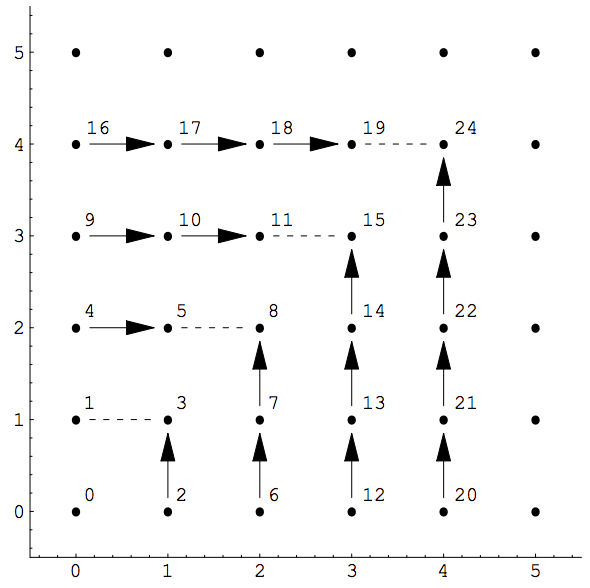
\includegraphics[width=\columnwidth]{Fig-Pairing.png}
  \end{minipage}

  Now please develop a mathematical formula for $\pi'$, (like the notation of original $\pi$),  and prove the correctness of your design.

\textbf{Solution:}

We can see that if the $x = 0, \pi'(0,y) = 0,1,4,9,... , y = 0,1,2,3...$

If the $y  = 0, \pi'(x,0) = 0,2,6,12... , x = 0,1,2,3...$

We define that $\pi'(x,y) = \begin{cases}  x+y^2 , &x < y \\ x(x+1)+y , & x \geq y \\ \end{cases} $

\textbf{Proof:}

First, we prove the function is a injective function, we assume two different pair $(x_1, y_1)$ and $(x_2,y_2)$.

We assume that $x_1<y_1,x_2<y_2$, so $\pi'(x_1,y_1) = x_1+y_1^2, \pi'(x_2,y_2) = x_2+y_2^2$, if $\pi'(x_1,y_1) = \pi'(x_2,y_2)$, we get $x_1-x_2 = (y_2+y_1)(y_2-y_1)$

If $x_1 = x_2$, $y_1 = y_2$, so we assume $x_1 >x_2$, then $y_2-y_1$ must equal to at least 1, and $y_2 +y_1 > x_1+x_2 > x_1-x_2$, so $x_1=x_2,y_1=y_2$

Similarily, we can prove the equlation is hold in other three conditions, so the function is injective.

Next, we prove the function is a surjective function, we can see that $ \forall z \in \mathbb{N}$,we can find $n \in \mathbb{N}$ that $n \leq z \leq (n+1)^2$

We assume $ m = z - n^2 $, if $ m < n $, then $(m,n)$ is the corresponding pair $(x,y)$, if $m \geq n$, then $(n,m-n)$ is the corresponding pair.

So, we've proved $\forall z \in \mathbb{N}$,there is a corresponding $(x,y)$, so the function is a surjective function.

So, our design is coorect.

\end{enumerate}


%========================================================================
\end{document}
